% !TeX root = ../cyh.tex

\chapter{内存管理组件开发与测试}

\section{开发过程}

本节主要介绍内存管理组件的开发过程,包括开发中遇到的困难以及相应的解决方案,并按时间顺序分为
前期准备、环境配置、基础实现和进阶开发四个部分。

\subsection{前期准备}

项目的第一到第六周是前期准备阶段,主要包括对 Rust 语言的学习、对操作系统内核的理解和对实验环境的准备。

Rust 语言是一种具有内存安全和并发性特点的系统级编程语言,因而
适合用于开发操作系统内核和系统调用接口。ArceOS 和 starry-next 都是基于 Rust 语言开发的,
因此在开发内存管理组件时,需要对 Rust 语言有一定的了解和掌握。
在本课题前期,我们参考了《Rust 语言升级》等相关资料,并结合操作系统训练营基础阶段的练习题目,深入学习了 Rust 语言的基本语法与特性。
其中,所有权、借用、生命周期等核心概念尤为重要,它们在支持操作系统内核的并发性和安全性方面发挥着关键作用。

在操作系统内核的学习方面,我们以 rCore-Tutorial 为例,学习如何实现一个简单的操作系统内核。
rCore-Tutorial-v3 是一个用 Rust 语言实现的以教学为目的的基本功能完备的操作系统,根据学习的顺序可分为九个章节:
实验环境配置、应用程序与基本执行环境、批处理系统、多道程序与分时多任务、地址空间、进程及进程管理、
文件系统与I/O重定向、进程间通信、并发,每个章节都有对应的代码分支和练习。跟随 rCore-Tutorial 的学习,
能够对操作系统的基本概念和实现有一个清晰的了解,为后续开发内存管理组件提供了基础。

同时,操作系统训练营的项目基础阶段详细介绍了 Unikernel 的搭建流程,
包括内存管理、任务调度、文件系统等组件的原理和实现方式,
以及如何基于 Unikernel 搭建宏内核,提供用户空间管理和 Linux 应用支持并进行相关的拓展。
这部分内容有助于加深对项目 starry-next 和基座 ArceOS 的理解。

\subsection{环境配置}

第七和第八周主要进行环境配置工作。为了验证 starry-next 内存管理模块及接口的设计与实现在 riscv64、x86\_64、loongarch64 和 aarch64 这四个架构下的正确性与性能,
我们使用了 qemu 模拟器来模拟这四个架构的运行环境,并且 qemu 模拟器的版本不应低于 8.2.0。qemu 是一个开源的虚拟机模拟器,支持多种硬件架构和操作系统,能够在主机上创建虚拟机并运行不同架构的操作系统。
同时,为了支持高版本的 qemu 模拟器,测例的本地运行都在 Ubuntu-24.04 下进行,并且需要在本地安装 rustling 工具链等 rust 相关工具,具体的操作可以参考项目的 README.md 文件。

另外,为了支持自动化测试,也为了探索合理高效宏内核开发模式,本课题不同方向的开发人员一同尝试了多种工具。
例如在项目初期使用 Gitlab 管理代码,并使用“全国大学生计算机系统能力大赛”平台进行测试,但由于平台的测试运行速度较慢且有时间限制,
因此转而使用 Github 进行代码管理,利用 GitHub Actions 进行自动化测试,定义了多个工作流配置文件,涵盖了不同架构和测试场景的自动化构建与验证。

\subsection{基础实现}

第九周到第十二周基础实现阶段的工作内容是完善宏内核基础功能,使其能够运行简单的 c 语言程序,
具体到内存管理方面,即实现 mmap、munmap、brk系统调用,完善内存管理组件的功能,并通过 basic 阶段的测例。
这一阶段中,测例反映出的问题主要分为三个层面:
\begin{itemize}
    \item 测例层面:测例本身存在问题,例如在 basic 阶段的 times 测例中,用于接受返回值的变量类型为 int 而非 man 手册中描述的 clock\_t,导致溢出,测例无法通过。
    \item starry-next 层面:宏内核的相关实现不完善,例如初始 mmap 系统调用接口的设计未完全参照 Linux 标准,构建新映射时没有取消旧映射。
    \item ArceOS 层面:ArceOS 相关组件或接口存在欠缺,例如在读取内存区域时范围错误等。
\end{itemize}

基础实现阶段的难点一是需要在开发中熟悉 Rust 语言和已有框架,二是要准确定位问题所在,因此需要掌握灵活的调试方法,
例如根据 starry-next 各个级别的日志信息进行调试,或者是使用 gdb 等工具。另外需要注意的是,
内存管理模块存在的问题可能会影响到其他模块的正常运行,例如在 clone 系统调用的实现中存在读取内存空间操作,
当启用 Lazy 映射时,会读取到未映射的内存区域,导致测例无法通过。因此,在开发中需要认识到测例集合的局限性,
并和其他模块的实现进行充分的沟通。

\begin{figure}
    \centering
    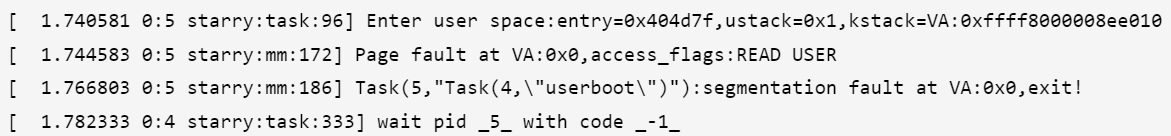
\includegraphics[width=0.8\linewidth]{page-fault-0x0-2.png}
    \caption{Lazy 映射下的缺页异常}
    \label{fig:page-fault-0x0}
\end{figure}

\subsection{进阶开发}

十三到十六周为进阶开发阶段,工作内容是完善内存管理组件的功能,使其能够支持更多的系统调用,如 mprotect、arch\_pctl、sysinfo、prlimit64 等,
并通过 libc-test 阶段的测例,同时,对于测例未覆盖的系统调用,也需要编写相应的测例。

在通过 libc-test 测例的过程中需要注意,不同架构下运行测例所需的系统调用可能不同,
例如在 x86\_64 架构下才会使用 fork 系统调用,其他三种架构下 fork 系统调用会被自动转换为 clone 系统调用。
同时,不同架构下对系统调用的实现细节也有不同的要求,例如在 clone 系统调用中,四个架构的参数传递顺序不完全相同,
其中 x86\_64 和 loongarch64 中第五个参数为子进程 id,第六个为 TLS,但在其他架构中二者的顺序相反。
因此,在进行调试或者编写测例时,需要根据具体的架构和系统调用要求进行调整。

\begin{lstlisting}[caption=不同架构下 clone 的部分参数传递顺序]
#[cfg(any(target_arch = "x86_64", target_arch = "loongarch64"))] child_tid: usize,
tls: usize,
#[cfg(not(any(target_arch = "x86_64", target_arch = "loongarch64")))] child_tid: usize,
\end{lstlisting}

本阶段测例涉及的系统调用较多,对各系统调用的实现完成度也有所不同。
在开发的过程中,会存在部分其他子系统的系统调用还未实现导致测例无法通过的情况,
但这些系统调用的具体功能并不需要实现,此时可以尝试通过令该系统调用直接返回成功的方式来绕过该问题。
但是对于 clone、mmap 等重要的系统调用,需要结合 man 手册和 DragonOS 等开源项目进行详细的实现。

在这一阶段中,比较常用的调试方法是观察 starry-next 各个级别的日志信息,
并和配合 qemu 模拟器和 strace 指令得到的系统调用信息进行对比,
以定位问题所在。

\begin{figure}
    \centering
    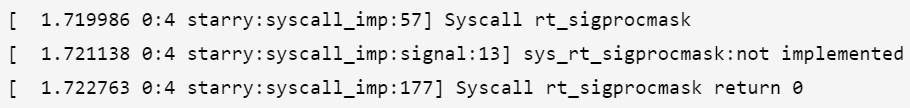
\includegraphics[width=0.8\linewidth]{return0-2.png}
    \caption{返回 0 绕过部分系统调用}
    \label{fig:return0}
\end{figure}

\section{内存管理组件的测试}

\subsection{测试用例分析}

测试用例分为两部分:开源测试用例和自定义测试用例。
其中开源测试用例主要来自 libc-test 库。libc-test 是一个针对 C 标准库(libc)功能及兼容性的检测工具。C 标准库作为 C 语言开发的基石,涵盖输入输出、内存管理、字符串操作等基础功能。
libc-test 借助一系列精心设计的测试用例,全面且细致地检验 C 标准库各功能模块,保障其在不同环境下的正确性和稳定性。在具体测试中,将编译完成的 libc-test 可执行文件作为输入,运行其中的静态与动态测试用例。
通过执行这些测试用例并检查输出结果,可判断待测内核是否能正确支持 C 标准库的各项功能,进而评估内核与 C 标准库的兼容性与稳定性。

尽管 libc-test 库提供了丰富的测试用例,可以涵盖大多数系统调用,例如 mmap、munmap、mprotect 等,但由于 libc-test 针对的是 C 标准库,而不是操作系统内核和系统调用的实现,
同时一部分系统调用无法使用 libc-test 进行测试,例如 sysinfo、prlimit64 等系统调用。
因此,我们还编写了一些自定义测试用例来验证 starry-next 内存管理模块的功能以及系统调用接口的正确性。这些用例将通过 C 标准库中 sys 子目录直接使用相关的系统调用,
并验证其返回值,例如:

\begin{lstlisting}[language=c, caption=直接使用系统调用进行测试的示例]
#include <sys/syscall.h>
syscall(SYS_write, fd, buf, len);
\end{lstlisting}

在测例的编写和运行过程中,strace 指令可以帮助我们跟踪系统调用的执行情况,在 Ubuntu-24.04 下通过 strace 指令可以得到 x86\_64 架构下的系统调用信息,
使用 qemu 模拟器配合 strace 指令也可以得到其他架构下的系统调用信息。
这些不仅可以帮助验证测例的正确性,还可以作为对照组可以帮助我们分析 starry-next 内存管理模块的实现是否符合 Linux 的标准实现,
以及系统调用的实现的正确性,从而进行进一步的调试和优化。

\subsection{测试用例实现}

【1】brk、mmap 和 munmap 系统调用:

在使用 malloc 等函数申请内存空间时,通常会先使用 brk 系统调用扩充堆空间,
然后再使用 mmap 系统调用进行内存映射,释放空间时则会使用 munmap 系统调用。
此处以 libc-test 中的 malloc\_0 为例,
该测例使用 malloc 函数申请了三个大小为 0 的空间,分配相应指针,并检测三个指针的地址是否相同,
若不同则测例通过,然后使用 free 进行释放指针指向的内存空间,
该测例可以检测 mmap 的匿名映射和 munmap 的释放是否正确。

另一方面,我们通过自定义测试用例来验证 mmap 系统调用文件映射的正确性,例如:
\begin{lstlisting}[caption=自定义 mmap 测例中调用 mmap 进行文件映射]
fd = open("test_mmap.txt", O_RDWR | O_CREATE);
array = mmap(NULL, kst.st_size, PROT_WRITE | PROT_READ, MAP_FILE | MAP_SHARED, fd, 0);
printf("mmap content: %s\n", array);
\end{lstlisting}

该测试用例打开了一个内容为“Hello, mmap successfully!”的文件,并使用 mmap 系统调用将该文件映射到内存中,然后读取文件内容,
如果能正确输出文件内容,则说明 mmap 系统调用的文件映射功能正常。

【2】mprotect 系统调用:

mprotect 系统调用用于修改指定内存区域的访问权限,在 libc-test 中常用于多线程及线程间通信的相关测例。
例如 pthread\_cond 测例测试了线程间通信的条件变量功能,需要使用 mprotect 系统调用将内存区域的访问权限修改为可读可写,
以保证线程间通信的正确性。

\begin{lstlisting}[caption= pthread\_cond 测例通过条件变量实现线程间通信]
TEST(r, pthread_mutex_init(&mtx, 0), "");
TEST(r, pthread_cond_init(&cond, 0), "");
TEST(r, pthread_mutex_lock(&mtx), "");
TEST(r, pthread_create(&td, 0, start_signal, (void *[]){ &cond, &mtx }), "");
TEST(r, pthread_cond_wait(&cond, &mtx), "");
TEST(r, pthread_join(td, &res), "");
TEST(r, pthread_mutex_unlock(&mtx), "");
TEST(r, pthread_mutex_destroy(&mtx), "");
TEST(r, pthread_cond_destroy(&cond), "");
\end{lstlisting}

【3】sysinfo 和 prlimit64 系统调用:

sysinfo 和 prlimit64 系统调用的自定义测试用例主要是通过获取系统信息和进程限制来验证其实现是否正确,
编写测例时需要注意二者的参数中都有特定的类型,例如 sysinfo 系统调用的参数类型为 sysinfo 结构体,
prlimit64 系统调用的参数类型为 rlimit 结构体。

\begin{lstlisting}[caption=prlimit64 测例部分代码]
#include <sys/syscall.h>
syscall(SYS_prlimit64, getpid(), RLIMIT_STACK, NULL, &old_limit);
\end{lstlisting}

\begin{lstlisting}[caption=sysinfo 测例部分代码]
#include <sys/sysinfo.h>
struct sysinfo info;
sysinfo(&info);
\end{lstlisting}

而 prlimit64 的最大文件数量限制则可以通过 libc-test 的 rlimit\_open\_files 测试用例来验证,
该测例会在设置资源限制后重复创建新的文件描述符(打开文件)至失败,并取当前最大文件描述符和资源限制值进行比较,相等则说明 prlimit64 系统调用能正常限制文件数量。

\begin{lstlisting}[caption=rlimit\_open\_files 测例设置资源限制并进行检验]
#include <sys/resource.h>
struct rlimit rl;
if (setrlimit(RLIMIT_NOFILE, &rl))
	t_error("setrlimit(%d, %ld) failed: %s\n", r, lim, strerror(errno));
if (getrlimit(RLIMIT_NOFILE, &rl))
	t_error("getrlimit(%d) failed: %s\n", r, strerror(errno));
if (rl.rlim_max != lim || rl.rlim_cur != lim)
	t_error("getrlimit %d says cur=%ld,max=%ld after setting the limit to %ld\n", r, rl.rlim_cur, rl.rlim_max, lim);
while((fd=dup(1)) != -1)
	if (fd > maxfd) maxfd = fd;
if (errno != EMFILE)
	t_error("dup(1) failed with %s, wanted EMFILE\n", strerror(errno));
if (maxfd+1 != lim)
	t_error("more fds are open than rlimit allows: fd=%d, limit=%d\n", maxfd, lim);
\end{lstlisting}


【4】性能测试

% 当前并未对 starry-next 内存管理模块的性能进行较完备的测试,
% 但在功能测试中,部分测例的运行时间也可以作为性能测试的参考。
% 我们将 starry-next 内存管理模块的性能与 Linux 的标准实现进行对比,
% 以验证 starry-next 内存管理模块的性能是否符合 Linux 的标准实现。

% 同时,还可以设计一些简单的测试用例,通过观察重复进行系统调用和内存操作所需的时间,
% 来评估 starry-next 内存管理模块的性能。例如:

当前并未对 starry-next 内存管理模块的性能进行较完备的测试,
但重复使用系统调用和内存读写的方式,也可以在一定程度上评估 starry-next 内存管理模块的性能。
因此设计测例,分别进行 1000 次 mmap、mummap、mprotect 和读写操作,
观察各架构单核和四核下的运行时间,并与运行在 qemu 模拟器下的 Linux 标准实现进行对比。

\begin{lstlisting}[caption=性能测试测例的部分代码]
for (int i = 0; i < NUM_ALLOCS; i++) {
    ptrs[i] = mmap(NULL, ALLOC_SIZE, PROT_READ | PROT_WRITE, MAP_PRIVATE | MAP_ANONYMOUS, -1, 0);
}
\end{lstlisting}

\subsection{测试结果与分析}

【1】brk、mmap 和 munmap 系统调用:

清单\ref{lst:malloc0}中展示了 malloc\_0 测试的结果,可以看到程序先调用 brk 系统调用拓展了堆空间,
调用了一次 mmap 系统调用为拓展的空间建立映射,length 为十六进制的 0x1000,
说明分配了一个页(4096字节)的内存空间,这是分配的最小单位。但因为 malloc 申请空间的大小为 0,
所以在第二和第三次 malloc 时空间足够,没有触发新的 mmap 系统调用,
之后 free 释放时也只调用了一次 munmap 系统调用。最终测例通过,匿名映射和映射解除功能正常。

\begin{lstlisting}[caption=运行 malloc\_0 测例的部分输出(info 级信息), label=lst:malloc0]
========== START entry-static.exe malloc_0 ==========
[  7.927777 1:11 starry::syscall:13] Syscall brk
[  7.930924 1:11 starry::syscall:211] Syscall brk return 1073741824
...
[  7.946120 1:11 starry::syscall:13] Syscall mmap
[  7.950708 1:11 starry_api::imp::mm::mmap:85] sys_mmap: addr: 40000000, length: 1000, prot: MmapProt(0x0), flags: MmapFlags(PRIVATE | FIXED | ANONYMOUS), fd: -1, offset: 0
[  7.972843 1:11 starry::syscall:211] Syscall mmap return 1073741824
...
[  8.022895 1:11 starry::syscall:13] Syscall munmap
[  8.028983 1:11 starry::syscall:211] Syscall munmap return 0
...
Pass!
========== END entry-static.exe malloc_0 ==========
\end{lstlisting}

自定义 mmap 测试用例的结果如清单\ref{lst:test_mmap}所示,可以看到程序成功读取到了文件中的内容,
说明文件映射功能正常。

\begin{lstlisting}[language=bash, caption=自定义 mmap 测例运行结果, label=lst:test_mmap]
========== START test_mmap ==========
file len: 27
mmap content:   Hello, mmap successfully!
========== END test_mmap ==========
\end{lstlisting}

【2】mprotect 系统调用:

清单\ref{lst:pthread-cond}中展示了 pthread\_cond 测例的结果,可以看到程序先调用 mmap 系统调用分配了一段内存空间,
由于 Lazy 映射的特性,这段内存空间并没有被映射到物理内存中,并且保护属性为空。
调用 mprotect 系统调用后,这段空间被分配了对应的物理地址,并且保护属性为可读可写,
说明 mprotect 系统调用的功能正常。

\begin{lstlisting}[caption=运行 pthread\_cond 测例的部分输出(info 级信息), label=lst:pthread-cond]
[  6.315702 3:11 starry::syscall:13] Syscall mmap
[  6.319449 3:11 starry_api::imp::mm::mmap:86] sys_mmap: addr: 0, length: 23000, prot: MmapProt(0x0), flags: MmapFlags(PRIVATE | ANONYMOUS), fd: -1, offset: 0
[  6.326679 3:11 starry::syscall:211] Syscall mmap return 667648
[  6.330263 3:11 starry::syscall:13] Syscall mprotect
[  6.333987 3:11 starry_api::imp::mm::mmap:169] sys_mprotect: addr: a5000, length: 21000, prot: MmapProt(READ | WRITE)
[  6.340052 3:11 starry_api::imp::mm::mmap:178] page not mapped
[  6.352141 3:11 starry_api::imp::mm::mmap:185] after sys_mprotect: paddr: PA:0x8140d000, flags: READ | WRITE | USER
[  6.357734 3:11 starry::syscall:211] Syscall mprotect return 0 
\end{lstlisting}

【3】sysinfo 和 prlimit64 系统调用:

% \begin{figure}
%     \centering
%     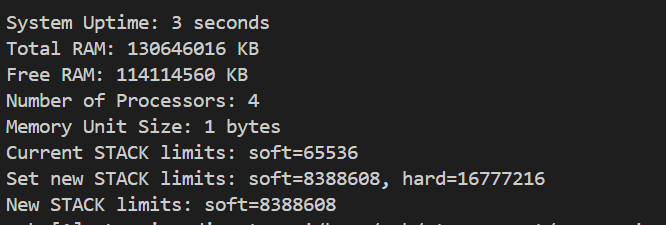
\includegraphics[width=0.5\linewidth]{sysinfo.png}
%     \caption{sysinfo 和 prlimit64 测试结果}
%     \label{fig:sysinfo-test}
% \end{figure}

从图\ref{fig:sysinfo-test}中可以看到,sysinfo 系统调用返回了系统信息,
例如当前系统共有 4 各处理器,系统运行时间为 3 秒,总内存为 130646016 KB,剩余内存为 114114560 KB。
prlimit64 系统调用则返回了进程用户栈的限制信息,
并且在设置用户栈大小时,prlimit64 系统调用正确使用了新的软限制值,
这说明 sysinfo 和 prlimit64 系统调用设置用户栈的功能正常。
同时,如图\ref{fig:prlimit64-test}所示,rlimit\_open\_files 测例也是通过的,
这说明 prlimit64 系统调用的文件数量限制功能正常。

\begin{figure}[H]
    \centering  % 图片全局居中
    \begin{subfigure}[t]{0.45\textwidth}
        \centering
        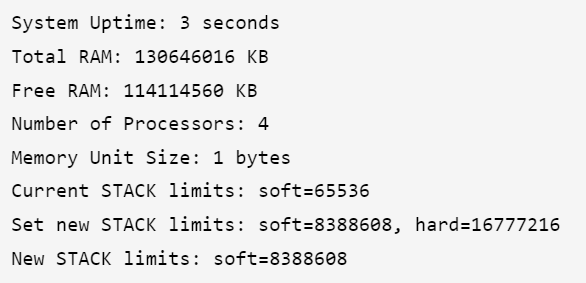
\includegraphics[width=\linewidth]{sysinfo-2.png}
        \caption{sysinfo 和 prlimit64 测试结果}
        \label{fig:sysinfo-test}
    \end{subfigure}
    \hfill % 添加一些水平间距
    \begin{subfigure}[t]{0.45\textwidth}
        \centering
        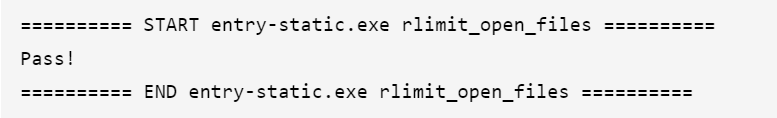
\includegraphics[width=\linewidth]{prlimit64-2.png}
        \caption{rlimit\_open\_files 测例结果}
        \label{fig:prlimit64-test}
    \end{subfigure}
    \caption{sysinfo 和 prlimit64 测试结果}
    \label{Fig.main3}
\end{figure}
% \begin{figure}
%     \centering
%     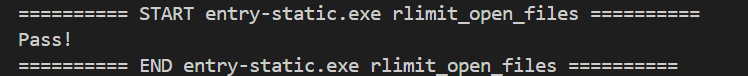
\includegraphics[width=0.5\linewidth]{prlimit64.png}
%     \caption{rlimit\_open\_files 测例结果}
%     \label{fig:prlimit64-test}
% \end{figure}



【4】性能测试:

% x86\_64 架构下,功能测试中的自定义 mmap 测例在 Linux 和 starry-next 上的运行时间
% 如图\ref{Fig.main}所示,starry-next 的运行时间远高于本机的运行时间。
% 同时,由图\ref{Fig.main2}可见starry-next 在映射、解除映射、读取和写入数据等方面花费的时间远高于 Linux 的运行时间,
% 尽管 starry-next 的运行还要受到 qemu 模拟器的影响,自身也实现了 Lazy Map 等内存管理方面的优化机制,
% 但总体来说,其性能仍有很大的提升空间。

% \begin{figure}[H]
%     \centering  % 图片全局居中
%     \begin{subfigure}[t]{0.45\textwidth}
%         \centering
%         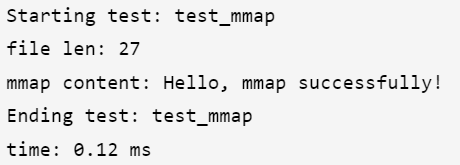
\includegraphics[width=\linewidth]{s2-local-2.png}
%         \caption{Linux}
%         \label{fig:sub.1}
%     \end{subfigure}
%     \hfill % 添加一些水平间距
%     \begin{subfigure}[t]{0.45\textwidth}
%         \centering
%         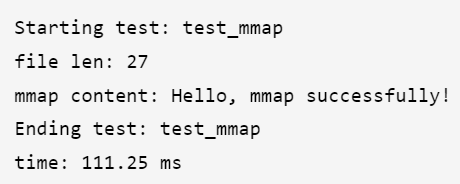
\includegraphics[width=\linewidth]{s2-starry-2.png}
%         \caption{starry-next}
%         \label{fig:sub.2}
%     \end{subfigure}
%     \caption{自定义 mmap 测试用例的运行时间对比}
%     \label{Fig.main}
% \end{figure}

% \begin{figure}[H]
%     \centering  % 图片全局居中
%     \begin{subfigure}[t]{0.45\textwidth}
%         \centering
%         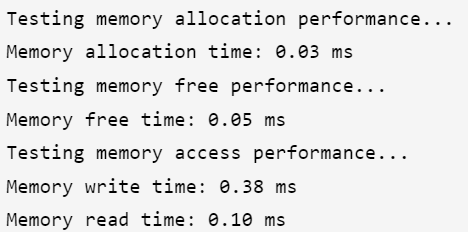
\includegraphics[width=\linewidth]{s1-2.png}
%         \caption{Linux}
%         \label{fig:sub.3}
%     \end{subfigure}
%     \hfill % 添加一些水平间距
%     \begin{subfigure}[t]{0.45\textwidth}
%         \centering
%         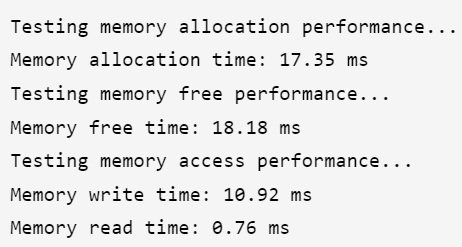
\includegraphics[width=\linewidth]{s1-starry-2.png}
%         \caption{starry-next}
%         \label{fig:sub.4}
%     \end{subfigure}
%     \caption{重复进行系统调用的运行时间对比}
%     \label{Fig.main2}
% \end{figure}


各架构下,单核和四核的运行时间如表\ref{tab:time-smp1}和表\ref{tab:time-smp4}所示。
可以观察到,各架构的运行时间相差较大,
这可能是由不同架构使用的页表结构、虚实地址结构、寻址方式等内存管理机制不同导致的,
同时,不同架构使用的交叉编译工具链对于程序编译、链接、优化方式的影响也可能导致运行时间的差异。
另外,四核下运行时间大于或等于单核的运行时间,可能是测例代码未充分使用多核的特性,
加上多核使得内核空间管理开销增加所致。

\begin{table}
    \centering
    \caption{各架构单核运行 1000 次操作的运行时间(单位:ms)}
    \begin{tabular}{ccccc}
        \toprule
        架构 & x86\_64 & LoongArch64  & RISC-V 64  & AArch64  \\ 
        \midrule
        mmap & 59.49 & 96.01 & 166.32 & 358.3 \\
        munmap & 244.17 & 1107.39 & 586.18 & 735.41 \\
        mprotect & 54.06 & 552.82 & 498.47 & 387.09 \\ 
        写 & 82.17 & 576.72 & 487.73 & 314.1 \\ 
        读 & 13.93 & 19.55 & 18.38 & 17.59 \\ 
        \bottomrule
    \end{tabular}
    \label{tab:time-smp1}
\end{table}

\begin{table}
    \centering
    \caption{各架构四核运行 1000 次操作的运行时间(单位:ms)}
    \begin{tabular}{ccccc}
        \toprule
        架构 & x86\_64 & LoongArch64  & RISC-V 64  & AArch64  \\ 
        \midrule
        mmap & 57.05 & 106.56 & 106.56 & 387.46  \\
        munmap & 259.87 & 1110.76 & 1110.76 & 804.91  \\
        mprotect & 54.06 & 552.82 & 498.47 & 387.09 \\ 
        写 & 81.73 & 592.46 & 592.46 & 443.21  \\
        读 & 11.15 & 20.16 & 20.16 & 18.7  \\
        \bottomrule
    \end{tabular}
    \label{tab:time-smp4}
\end{table}

% \begin{table}
%     \centering
%     \caption{各架构四核运行 1000 次 mmap、mummap、mprotect 和读写操作的运行时间(单位:ms)}
%     \begin{tabular}{ccccccccc}
%         \toprule
%         架构 & x86\_64 & x86\_64 & LoongArch64 & LoongArch64 & RISC-V 64 & RISC-V 64 & AArch64 & AArch64  \\ 
%         \midrule
%         mmap & 59.49 & 57.05 & 96.01 & 106.56 & 166.32 & 185.35 & 358.3 & 387.46 \\
%         munmap & 244.17 & 259.87 & 1107.39 & 1110.76 & 586.18 & 722.97 & 735.41 & 804.91 \\
%         mprotect & 54.06 & 50.26 & 552.82 & 561.13 &  498.47 & 511.25 & 387.09 & 532.12  \\ 
%         写 & 82.17 & 81.73 & 576.72 & 592.46 & 487.73 & 480.99 & 314.1 & 443.21 \\ 
%         读 & 13.93 & 11.15 & 19.55 & 20.16 & 18.38 & 18.55 & 17.59 & 18.7 \\ 
%         \bottomrule
%     \end{tabular}
%     \label{tab:time-smp4}
% \end{table}

另一方面,如图\ref{Fig.main2}所示,以 x86\_64 架构下的结构为例,starry-next 在内存读写方面的性能和 Linux 相近,
但是系统调用方面的性能低于 Linux,这可能是由于二者在页表结构、寻址方式等方面相似,
但是 Linux 提供了更多页面映射和管理的优化,例如提供了更灵活的页面置换算法等。


\begin{figure}[H]
    \centering  % 图片全局居中
    \begin{subfigure}[t]{0.45\textwidth}
        \centering
        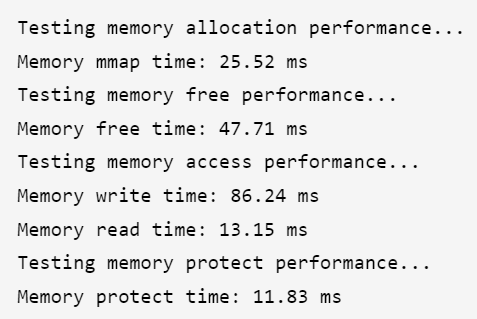
\includegraphics[width=\linewidth]{speed-linux.png}
        \caption{Linux}
        \label{fig:sub.3}
    \end{subfigure}
    \hfill % 添加一些水平间距
    \begin{subfigure}[t]{0.45\textwidth}
        \centering
        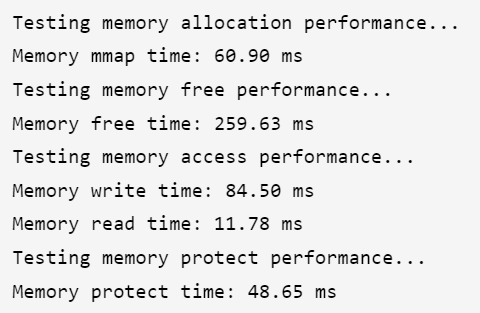
\includegraphics[width=\linewidth]{speed-starry.png}
        \caption{starry-next}
        \label{fig:sub.4}
    \end{subfigure}
    \caption{重复1000次各操作运行时间对比}
    \label{Fig.main2}
\end{figure}

